\documentclass[letterpaper,10pt,onecolumn,draftclsnofoot]{IEEEtran}
\usepackage{times}

\usepackage[english]{babel}
\usepackage[margin=0.75in]{geometry}

\usepackage{graphicx}

\DeclareGraphicsExtensions{.pdf,.png,.jpg}

\title{Object speed Tracking}
\author{Alex Bailey, Ben Wick, Dylan Washburne\\CS 461, Fall Term}

\begin{document}

\begin{titlepage}

\maketitle

\begin{abstract}
Using a stationary camera, with the intent of being mounted on a car, we are attempting to  detect objects and determine the speeds of those objects relative to the Observer (camera).
This will be done by having the camera recognize objects in space and determine their speeds based on the rate at which they travel through the frame.
If the camera is on a moving object, then we will need to either have a way for the system to measure it's own speed, likely with an accelerometer or connect to the object, if the object is measuring it's own speed.
To make this work, we will have to research the varieties of cameras available to use, as well as the API’s  they operate with.
We will also have to review the available computer vision algorithms and determine which is the most appropriate.
From this, we will determine the best camera to be used and from there create a object tracking program.
 
\end{abstract}

\end{titlepage}

\section{Problem Definition}

There are many applications for tracking the speeds of moving objects.
Some examples include tracking the speed of a vehicle for use by law enforcement, tracking the speed of groups of people for use in analyzing group movement, and tracking sports players during practice.
However, the current methods of tracking objects have too many drawbacks to make them acceptable anymore. 
There is a need for a new system that can track the speeds of moving objects that doesn't have these drawbacks.


Primary among these problems is that radar and similar methods perform poorly in poor weather conditions.
These methods also put out a detectable signal that can be used to exploit weaknesses in law enforcement tactics , are incapable of tracking more than one object at a time, requires a trained user actively operating the device, and have problems with accuracy (eg. if the user misses the target there will be no reading or the user may not be certain that the reading on the device came from the intended target).

 In our modern society, these shortcomings are no longer acceptable.
 We have used the methods provided to us because there were no other options to work with.


%Distance is maybe an issue to look for

\section{Proposed Solution}

We are going to use a camera and a computer vision program to identify objects and to track the speed of passing objects.
 The system will be able to track passing objects and display their current speeds to the user.
 The system will also be able to accurately detect the speeds of passing objects during inclement weather conditions, such as heavy rain, in which other methods would return bad results.
 The camera and computer vision software to be used is yet to be determined, however we can select the camera and computer vision software to use by examining the strengths and shortcomings presented.
 After selecting a camera and computer vision software, we will work to incorporate the computer vision software with the camera’s api to determine object recognition.
 From there, we will gauge the object’s speed based on its movement in-frame, so that we can return instantaneous results to the user.
 

\section{Performance Metrics}

Our solution will be able to identify and detect nearby objects which can be tracked.
After the initial setup, the system will not need user input until the user chooses to terminate the program.
The system will be able simultaneously process the speed of at least 6 objects on screen. 
When the system identifies something as an object, at least 70\% of the time, this will be the desired object type.
The system will then track the nearby object to determine speed, and return the value within 10\% of its actual speed.
The system will be able to process the information and display it to the user within 0.5 seconds of it being recognized.

 
%Applications somewhere maybe

\hfill \break

\hfill \break

\hfill \break



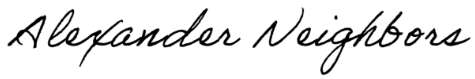
\includegraphics[scale=0.5]{signature}

\end{document}
